\begin{figure}[H]
    \centering
    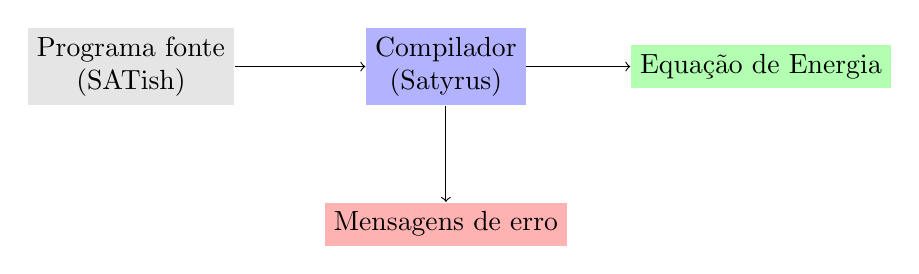
\begin{tikzpicture}[nodes={fill=gray!20}, row sep=0.3cm,column sep=0.5cm]
        \node[rectangle, align=center] (input) at (0,0) {Programa fonte \\ (SATish)};
        \node[rectangle, fill=blue!30, align=center] (compiler) at (4, 0) {Compilador \\ (Satyrus)};
        \draw[->] (input) to[out=0,in=180] (compiler);
        \node[rectangle, fill=green!30] (target) at (8, 0) {Equação de Energia};
        \draw[->] (compiler) to[out=0,in=180] (target);
        \node[rectangle, fill=red!30] (error) at (4, -2) {Mensagens de erro};
        \draw[->] (compiler) to (error);
    \end{tikzpicture}
    \label{fig:compiler-flow}
    \caption{A estrutura básica de um compilador.}
\end{figure}